\def\docroot{..}
\documentclass[\docroot/reports/draft/report.tex]{subfiles}

\begin{document}

\onlyinsubfile{\tableofcontents}

Гравитация в метрике Шварцшильда хорошо изучена. В данной метрике решалась масса различных задач о гравитационных волнах, их взаимодействии с электромагнитными волнами и веществом. Скалярные и электромагнитные волны сами по себе до сих пор обходились стороной. Однако понимание структуры более простых полей (скалярного, векторного) в метрике Шварцшильда может быть полезно при анализе более сложных (тензорных) полей.

Поскольку пространство Шварцшильда обладает теми же симметриями, что и пространство Минковского, угловые части сферических гармоник в метрике Шварцшильда и метрике Минковского совпадают. Отыскание сферических гармоник в метрике Шварцшильда сводится к отысканию лишь радиальных частей для отдельных компонент гармоник.

Из-за нетривиальной структуры пространства, однако, радиальные части искомых решений очень сложны и задаются своими дифференциальными уравнениями, получающимися в результате разделения переменных в вариационных уравнениях. Зависимость от времени полагается известной ($\exp(- i \omega t)$). Выражение решений в аналитическом виде сопряжено с большими трудностями, поскольку получаемые в результате разложения в окрестности особых точек ряды не сводятся к известным рядам простыми преобразованиями.

В данном разделе производится предварительный анализ задающих уравнений с целью определения подходящих начальных условий для численной процедуры решения. Полученные решения сравниваются с решениями в плоском пространстве, анализируются плотность и поток энергии.

\subsection{Скалярное поле}\label{sec:scal}

    Рассмотрим скалярное поле $f(t,r,\theta,\phi)$. В общем случае ему соответствует лагранжиан (в четырехмерной нотации)
    %
    \begin{equation*}
        \mathcal{L} = \frac{1}{2} g^{ij} f_{,i} f_{,j}.
    \end{equation*}
    %
    Поскольку $f$~--- скалярное поле, выражения $f_{,i}$ и $f_{;i}$ эквивалентны, и лагранжиан может быть переписан в виде
    %
    \begin{equation*}
        \mathcal{L} = \frac{1}{2} g^{ij} f_{;i} f_{;j}.
    \end{equation*}
    %
    В этой форме особенно легко получить вариационное уравнение:
    %
    \begin{equation*}
        g^{ij} f_{;ij} = 0.
    \end{equation*}

    Несложно показать, применяя одну из методик разделения переменных (например, метод Ли-генерации сферических гармоник \cite{burlankov_tmf, burlankov_space_dynamics,BurVas2019}), что поле $f$ должно представляться в виде
    %
    \begin{equation*}
        f(t,r,\theta,\phi) = Y_l^m(\theta,\phi) F(t,r)
    \end{equation*}
    %
    для любого сферически-симметричного пространства. Сферические функции $Y_l^m(\theta,\phi)$ известны из общей теории математической физики. Ненормированные сферические функции имеют вид:
    %
    \begin{equation*}
        Y_l^m(\theta,\phi) = e^{im\phi} P_l^m(\cos\theta),
    \end{equation*}
    %
    где $P_l^m(\cos\theta)$~--- присоединенные полиномы Лежандра.

    Выбирая зависимость от времени пропорциональной $e^{-i \omega t}$, что обычно естественно для волновых нестатических решений, а также рассматривая лишь основную гармонику с $m = 0$, приходим к следующему виду основной гармоники, который мы и будем далее исследовать подробно:
    %
    \begin{equation*}
        f(t,r,\theta) = e^{-i \omega t} w(r) P_l^m(\cos\theta).
    \end{equation*}
    %
    Без потери общности константу $\omega$ можно положить равной единице, чем мы и будем пользоваться для краткости и удобства.

    Тензор энергии-импульса для скалярного поля элементарно получается из лагранжиана. Записанный в более наглядной ковариантной форме, он выглядит следующим образом:
    %
    \begin{equation*}
        \mathcal{T}_{ij} = \frac{1}{2} \qty(- g_{ij} f^{,s} f_{,s} + 2 f_{,i} f_{,j}) .
    \end{equation*}
    %
    В силу симметричности $g_{ij}$, он уже является симметричным. Следуя ранее озвученному замечанию, запишем выражение для среднего по периоду тензора энергии-импульса:
    %
    \begin{equation*}
        \mathcal{T}_{ij} = \frac{1}{4} \mathop{\mathrm{Re}}\qty{- g_{ij} f^{,s} f^*_{,s} + 2 f_{,i} f^*_{,j}} .
    \end{equation*}

    \paragraph{Плоское пространство.}

        Найдем вид неизвестной функции $w(r)$ в плоском пространстве.

        Подставляя в вариационное уравнение основную гармонику и выбирая метрику Минковского в качестве метрики пространства, приходим к дифференциальному уравнению, в котором угловая, временн\'{а}я и радиальная части разделяются. Уравнение для радиальной части принимает вид:
        %
        \begin{equation}\label{eq:scal-m-eq}
            r^2 w''(r) + 2 r w'(r) + (l\,(l+1) - r^2) w(r) = 0.
        \end{equation}
        %
        Решениями данного уравнения являются сферические функции Бесселя $y_l(r)$ и $j_l(r)$, которые при $r\to\infty$ ведут себя как (затухающие) $\sin(r)$ и $-\cos(r)$ (при $l = 0$; при других $l$ у функций появляется общая дополнительная фаза) соответственно.

        Функция $F(r,t) = \exp(-i t) w(r)$ (см. замечание о $\omega = 1$) в обоих случаях описывает стоячую волну с узлами в нулях функции $w(r)$. Это следствие комплексного представления искомого решения. Для описания бегущих волн достаточно произвести следующую манипуляцию. Из чисто действительных функций $y_l(r)$ и $j_l(r)$ можно скомпоновать комплексные функции $h^{1,2}_l = j_l(r) \pm i\,y_l(r)$, известные как сферические функции Ганкеля первого и второго рода (\autoref{fig:scal-h12}), переходящие на бесконечности в (убывающие) комплексные экспоненты $e^{\pm i r}$. Их сумма и разность, очевидно, опять приводят к стоячим решениям.
        %
        \begin{figure}[h]
            \centering
            %
            \subfloat[][]{%
                \label{fig:scal-h1}%
                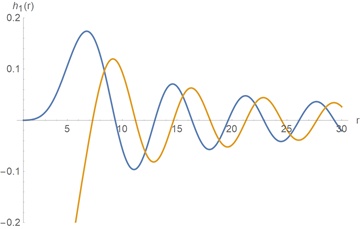
\includegraphics[width=0.45\textwidth]{scal-vec/scal-h1}}%
            \hspace{8pt}%
            %
            \subfloat[][]{%
                \label{fig:scal-h2}%
                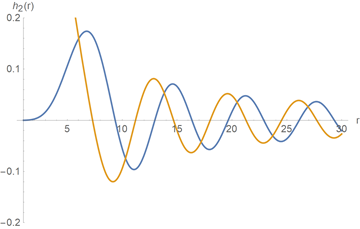
\includegraphics[width=0.45\textwidth]{scal-vec/scal-h2}}%
            \hspace{8pt}%
            %
            \caption[]{Сферические функции Ганкеля $h^{1,2}_l$ ($l=5$) \subref{fig:scal-h1} первого и \subref{fig:scal-h1} второго рода. Изображены действительная и мнимая части}%
            \label{fig:scal-h12}%
        \end{figure}

        Плотность энергии бегущих волн в общем случае не монотонна по радиусу (\autoref{fig:scal-ee}). Сначала она быстро убывает от значения бесконечности при $r = 0$ до своего минимального значения, затем монотонно выходит на постоянный уровень при $r \to \infty$. Поток энергии имеет только радиальную составляющую, от $r$ не зависящую. У стоячих волн, в отличие от бегущих, плотность энергии при $r = 0$ равна нулю. Кривая плотности сильно осциллирует. Среднее значение плотности энергии выходит на постоянный уровень при $r \to \infty$. Поток энергии в этом случае отсутствует.
        %
        \begin{figure}[h]
            \centering
            %
            \subfloat[][]{%
                \label{fig:scal-h1-ee-p2}%
                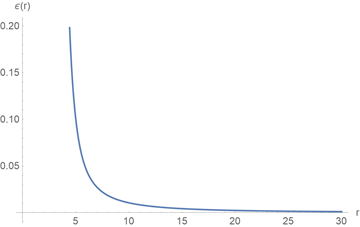
\includegraphics[width=0.45\textwidth]{scal-vec/scal-h1-ee-p2}}%
            \hspace{8pt}%
            %
            \subfloat[][]{%
                \label{fig:scal-j1-ee-p2}%
                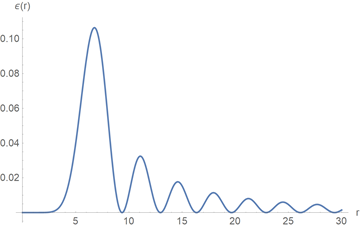
\includegraphics[width=0.45\textwidth]{scal-vec/scal-j1-ee-p2}}%
            \hspace{8pt}%
            %
            \subfloat[][]{%
                \label{fig:scal-h1-ee}%
                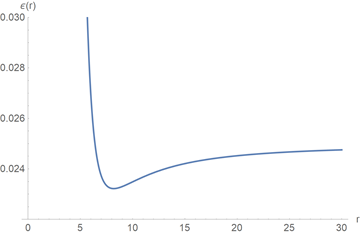
\includegraphics[width=0.45\textwidth]{scal-vec/scal-h1-ee}}%
            \hspace{8pt}%
            %
            \subfloat[][]{%
                \label{fig:scal-j1-ee}%
                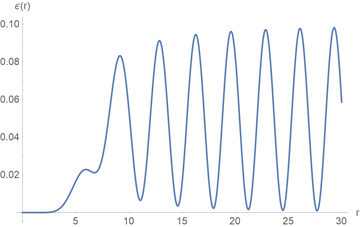
\includegraphics[width=0.45\textwidth]{scal-vec/scal-j1-ee}}%
            \hspace{8pt}%
            %
            \caption[]{Плотность энергии $l=5$ моды бегущей (\subref{fig:scal-h1-ee-p2}, \subref{fig:scal-h1-ee}) и стоячей (\subref{fig:scal-j1-ee-p2}, \subref{fig:scal-j1-ee}) волн в зависимости от радиуса при фиксированных углах $\theta = \pi/2$ и $\theta = \pi/4$}%
            \label{fig:scal-ee}%
        \end{figure}

        Сравнительный анализ вида функции $F(r,t)$ в разных метриках, а также плотности и потока энергии произведем после обсуждения решения вариационных уравнений в метрике Шварцшильда.

    \paragraph{Метрика Шварцшильда.}

        Уравнение для радиальной части принимает вид:
        %
        \begin{gather}\label{eq:scal-sw-eq}
            w''(r) + \qty(\frac{1}{r} + \frac{1}{r - r_g})\, w'(r) - \qty(\frac{l\,(l+1)}{r\, (r-r_g)} - \frac{r^2}{(r-r_g)^2})\, w(r) = 0.
        \end{gather}
        %
        Оно достаточно к\'{о}мплексное, хотя, в отличие от векторного поля (кроме уравнения для последней компоненты), и не компл\'{е}ксное (не содержит в явном виде мнимой единицы). К сожалению, уже и оно не имеет решений в виде конечных комбинаций известных математических функций. То же относится и к аналогичном уравнениям для векторного поля.

        Получить его решение можно двумя путями: в виде ряда разложением в окрестности особых точек и численно. Для численного решения, однако, необходимо знать начальные условия. Помимо того, что характер уравнения в окрестности особых точек сам по себе представляет интерес, полученные решения могут помочь в выборе правильных начальных условий для численной процедуры решения. Численное решение же, будучи известным при всех значениях $r$, а не только в окрестности, позволит наглядно исследовать плотность и поток энергии.

        Уравнение (\ref{eq:scal-sw-eq}), в отличие от аналогичного уравнения в плоском пространстве, имеет две регулярные особые точки, $r = 0$ и $r = r_g$, плюс обычную для уравнений такого типа особую точку $r = \infty$. Решения в окрестности регулярных особых точек сходятся соответственно на интервалах $(0,\,r_g)$ и $(0,\,2r_g)$.

        Представим исследуемое уравнение в виде (\ref{eq:deq_init}) в окрестности $r = 0$, откуда определим $p(r)$ и $q(r)$:
        %
        \begin{equation*}
            p(r) = 1 + \frac{r}{r - r_g}, \qquad
            q(r) = -\frac{l\,(l+1)\,r}{r-r_g} + \frac{r^4}{(r-r_g)^2} .
        \end{equation*}
        %
        Характеристическое уравнение для особой точки $r = 0$ принимает вид:
        %
        \begin{equation*}
            \lambda^2 + (p_0 - 1) \lambda + q_0 = 0, \qquad
            p_0 = 1, \qquad q_0 = 0 ,
        \end{equation*}
        %
        откуда $\lambda_{1,2} = 0$. Первое общее решение для данной окрестности приобретает вид степенного ряда общего вида:
        %
        \begin{equation*}
            w(r) = 1 + \sum\limits_{n = 1}^\infty w_n r^n ,
        \end{equation*}
        %
        где коэффициенты определяются последовательно из (\ref{eq:deq_coefs}).

        К сожалению, вид коэффициентов $w_n$ получается слишком сложным для аналитического выражения. Анализ, однако, показывает, что коэффициенты $w_n$ можно представить в виде следующей суммы:
        %
        \begin{equation*}
            w_n = h_n + \omega_n,
        \end{equation*}
        %
        где $h_n$~--- коэффициенты разложения гипергеометрической функции ${}_2F_1(-l,\ l+1,\ 1;\ r / r_g)$, причем указанная функция является хорошим приближением для $w(r)$ вплоть до более чем середины области сходимости, а ближе к $r = r_g$ начинает серьезно отличаться (\autoref{fig:scal-r0-2f1-comp}). Коэффициенты $\omega_n$ не выражаются простым образом.
        %
        \begin{figure}[!htb]%
            \centering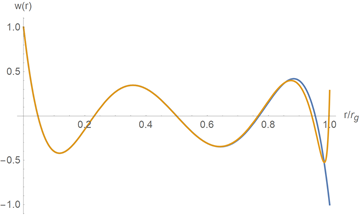
\includegraphics[width=0.45\textwidth]{scal-vec/scal-r0-2f1-comp}%
            \caption[]{Сравнение вида функций $w_l$ и ${}_2F_1$ при $l = 5$. Искомое решение продолжает осциллировать, плотно прижимаясь к вертикальной прямой $r = r_g$, в то время как гипергеометрическая функция сгибается вниз}%
            \label{fig:scal-r0-2f1-comp}%
        \end{figure}

        Второе решение в окрестности $r = 0$ можно получить по формуле (\ref{eq:deq_alt_sln}), однако без явного аналитического выражения коэффициентов первого из решений это достаточно проблематично. На самом деле нет необходимости искать второе решение в принципе, поскольку радиус сходимости решения в окрестности соседней регулярной особой точки полностью перекрывается с радиусом сходимости данного решения. У решений, однако, могут отличаться некоторые параметры (фаза), которые можно сопоставить отдельно для каждого $l$. Численный эксперимент показывает, что такая зависимость имеет неконстантную составляющую, близкую по форме к $l^{1/2}$ или $\log(l+1)$.

        Проделывая ту же процедуру в окрестности второй особой точки $r = r_g$, получим схожие, но более оптимистичные результаты:
        %
        \begin{equation*}
            p(r) = 2 - \frac{r_g}{r}, \qquad
            q(r) = -\frac{l\,(l+1)\,(r - r_g)}{r} + r^2 ,
        \end{equation*}
        %
        \begin{equation*}
            \lambda^2 + (p_0 - 1) \lambda + q_0 = 0, \qquad
            p_0 = 1, \qquad q_0 = r_g^2 ,
        \end{equation*}
        %
        откуда показатели особой точки $\lambda_{1,2}$ различны и не отличаются на действительную целую константу: $\lambda_{1,2} = \pm i r_g$. Здесь, увы, уже не так просто получить близкое аналитическое решение выделением известных рядов из $w(r)$, сами коэффициенты $w_n$ также существенно более сложные. Однако оба решения являются различными, что позволяет найти второе, недостающее решение в области $(0,\,r_g)$. Оба решения представляются следующими рядами:
        %
        \begin{equation*}
            w(r) = \qty(r-r_g)^{\pm i r_g} \qty(1 + \sum\limits_{n = 1}^\infty w_n (r - r_g)^n) .
        \end{equation*}

        Вид функций $w(r)$ анализируется далее при рассмотрении свойств решений.

    \paragraph{Свойства решений.}

        Разложение решения в ряд в окрестности $r = r_g$ является, очевидно, комплексным~--- в отличие от плоского пространства, решения здесь уже не могут быть чисто стоячими, однако они и не являются чисто бегущими. Обнаруживаются следующие свойства решений:
        %
        \begin{enumerate}
            \item При $r \gg r_g$ (\autoref{fig:scal-rg} \subref{fig:scal-rg-sec2}, \autoref{fig:scal-rg2} \subref{fig:scal-rg2-sec2}) действительные части обоих решений совпадают, мнимые части противоположны по знаку. Мнимая и действительная части каждого из решений с точностью до константы совпадают друг с другом, при этом мнимая часть всегда меньше по амплитуде. Доворотом фазы мнимую (эквивалентно, действительную) часть можно обратить в нуль. В силу этого, волны при $r \gg r_g$ стоячие. Более того, поскольку между мнимой и действительной частями решений нет (нетривиальной, т.е. не кратной $\pi$) разности фаз, получить бегущие волны линейной комбинацией решений невозможно. В этой части пространства решения напоминают сферические функции Бесселя первого рода (включая их убывание пропорционально первой степени $r$ при $r \to \infty$), однако в чистом виде ими не являются.
            %
            \item При $r = r_g + \varepsilon$ (\autoref{fig:scal-rg} \subref{fig:scal-rg-sec2-rg}, \autoref{fig:scal-rg2} \subref{fig:scal-rg2-sec2-rg}) для некоторого малого $\varepsilon > 0$ волны эффективно бегущие. Действительная и мнимая части ортогональны. Частота колебаний неограниченно возрастает при приближении к сингулярности (т.е. при движении в сторону уменьшения $\varepsilon$). Именно в этой части пространства, по сравнению с предыдущим случаем, наиболее выражен поток энергии (см. далее). Волны здесь, однако, очень слабые~--- их амплитуда на несколько порядков меньше амплитуды волн в области $r \gg r_g$.
            %
            \item Как и при $r = r_g + \varepsilon$, при $r = r_g - \varepsilon$ (\autoref{fig:scal-rg} \subref{fig:scal-rg-sec1-rg}, \autoref{fig:scal-rg2} \subref{fig:scal-rg2-sec1-rg}) в направлении сингулярности ($\varepsilon \to 0$) частота волн неограниченно возрастает. Волны здесь напоминают отраженные (относительно $r = r_g$), но измененные по масштабу волны в области $r = r_g + \varepsilon$.
            %
            \item При $r < r_g$  (\autoref{fig:scal-rg} \subref{fig:scal-rg-sec1}, \autoref{fig:scal-rg2} \subref{fig:scal-rg2-sec1}) волны чисто бегущие. Действительная и мнимая части решений полностью ортогональны. Сами решения напоминают при определенном сдвиге фазы гипергеометрическую функцию ${}_2 F_1$ (см. выше). Первое решение отличается от второго лишь масштабом и знаком мнимой части. Во всей данной области волны также очень слабы независимо от номера решения.
        \end{enumerate}
        %
        \begin{figure}[h]
            \centering
            %
            \subfloat[][]{%
                \label{fig:scal-rg-sec1}%
                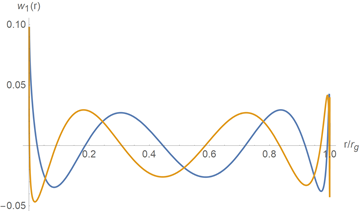
\includegraphics[width=0.45\textwidth]{scal-vec/scal-rg-sec1}}%
            \hspace{8pt}%
            %
            \subfloat[][]{%
                \label{fig:scal-rg-sec2}%
                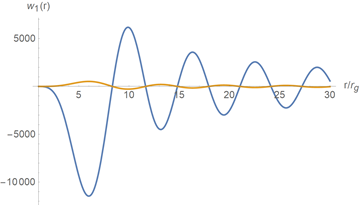
\includegraphics[width=0.45\textwidth]{scal-vec/scal-rg-sec2}}%
            \hspace{8pt}%
            %
            \subfloat[][]{%
                \label{fig:scal-rg-sec1-rg}%
                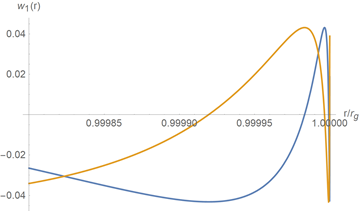
\includegraphics[width=0.45\textwidth]{scal-vec/scal-rg-sec1-rg}}%
            \hspace{8pt}%
            %
            \subfloat[][]{%
                \label{fig:scal-rg-sec2-rg}%
                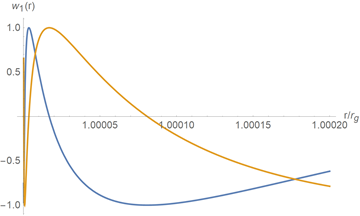
\includegraphics[width=0.45\textwidth]{scal-vec/scal-rg-sec2-rg}}%
            \hspace{8pt}%
            %
            \caption[]{Решение $w_1(r)$ ($l = 5$, действительная и мнимая части) в различных областях:
                \subref{fig:scal-rg-sec1}~$r<r_g$,
                \subref{fig:scal-rg-sec2}~$r > r_g$,
                \subref{fig:scal-rg-sec1-rg}~$r = r_g - \varepsilon$,
                \subref{fig:scal-rg-sec2-rg}~$r = r_g + \varepsilon$}%
            \label{fig:scal-rg}%
        \end{figure}
        %
        \begin{figure}[h]
            \centering
            %
            \subfloat[][]{%
                \label{fig:scal-rg2-sec1}%
                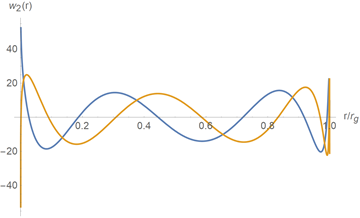
\includegraphics[width=0.45\textwidth]{scal-vec/scal-rg2-sec1}}%
            \hspace{8pt}%
            %
            \subfloat[][]{%
                \label{fig:scal-rg2-sec2}%
                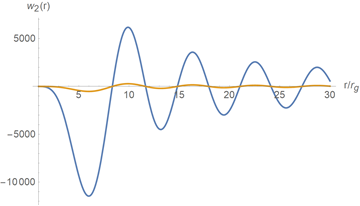
\includegraphics[width=0.45\textwidth]{scal-vec/scal-rg2-sec2}}%
            \hspace{8pt}%
            %
            \subfloat[][]{%
                \label{fig:scal-rg2-sec1-rg}%
                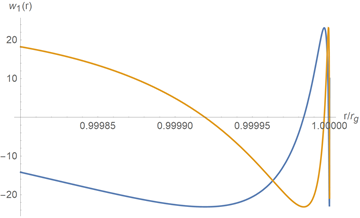
\includegraphics[width=0.45\textwidth]{scal-vec/scal-rg2-sec1-rg}}%
            \hspace{8pt}%
            %
            \subfloat[][]{%
                \label{fig:scal-rg2-sec2-rg}%
                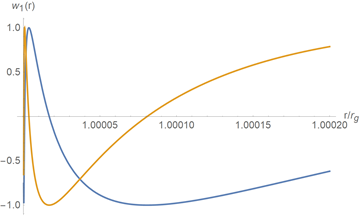
\includegraphics[width=0.45\textwidth]{scal-vec/scal-rg2-sec2-rg}}%
            \hspace{8pt}%
            %
            \caption[]{Решение $w_2(r)$ ($l = 5$, действительная и мнимая части) в различных областях:
                \subref{fig:scal-rg2-sec1}~$r<r_g$,
                \subref{fig:scal-rg2-sec2}~$r > r_g$,
                \subref{fig:scal-rg2-sec1-rg}~$r = r_g - \varepsilon$,
                \subref{fig:scal-rg2-sec2-rg}~$r = r_g + \varepsilon$}%
            \label{fig:scal-rg2}%
        \end{figure}
        %
        В целом, первое решение отличается от второго лишь масштабом левой части ($r < r_g$) и знаком мнимой части. Каждое из решений является как стоячей, так и бегущей волной в зависимости от области пространства. Любая линейная комбинация двух решений не может превратить волну в чисто бегущую или чисто стоячую во всем пространстве~--- область $r \gg r_g$ в любом случае будет содержать стоячую волну.

        Следует еще раз напомнить, что область сходимости решений в виде рядов в окрестности особых точек эффективно ограничена расстоянием от данной особой точки до ближайшей. Решения за пределами области сходимости $(0,2 r_g)$ можно получить численным интегрированием (отдельно слева и справа от особой точки) задающего дифференциального уравнения для функции $w(r)$ с начальными условиями, полученными в результате вычисления $w(r_0)$ и $w'(r_0)$ в некоторой точке из соответствующего интервала (левой или правой половины области сходимости). Разумно использовать только разложение в окрестности $r_g$, поскольку оно определено во всей области $(0,2 r_g)$.

        Поскольку уравнение несколько жесткое, следует внимательно относиться к выбору численной процедуры. Интегрирование производилось в пакете \foreignlanguage{english}{Wolfram Mathematica}. Параметры интегрирования, влияющие на точность решения, пришлось выбирать вручную исходя из анализа невязки, возникающей при подстановке найденного решения в исходное уравнение.

    \paragraph{Плотность и поток энергии.}

        У стоячих волн поток энергии отсутствует, а плотность энергии осциллирует в направлении изменения $r$ подобно самой волне. У бегущих волн поток должен асимптотически стремиться к константе. Также должна вести себя и плотность энергии.

        В случае с плоским пространством можно получить обе описанные картины, поскольку можно разделить бегущие и стоячие волны. В метрике Шварцшильда любая данная волна в зависимости от области пространства является стоячей или бегущей.

        Если рассматривать первоначальные решения, в которых в области $r > r_g$ волны содержат как стоячую, так и бегущую компоненты, можно получить следующую картину плотности и потока энергии (\autoref{fig:scal-ee-uu}, \autoref{fig:scal-ee-uu-p2}).
        %
        \begin{figure}[h]
            \centering
            %
            \subfloat[][]{%
                \label{fig:scal-rg-ee-sec1}%
                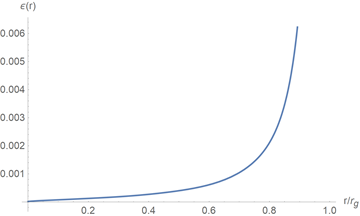
\includegraphics[width=0.45\textwidth]{scal-vec/scal-rg-ee-sec1}}%
            \hspace{8pt}%
            %
            \subfloat[][]{%
                \label{fig:scal-rg-uu-sec1}%
                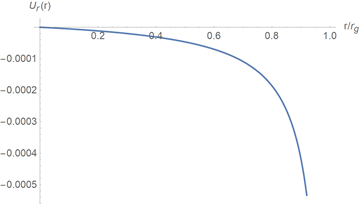
\includegraphics[width=0.45\textwidth]{scal-vec/scal-rg-uu-sec1}}%
            \hspace{8pt}%
            %
            \subfloat[][]{%
                \label{fig:scal-rg-ee-sec2-rg}%
                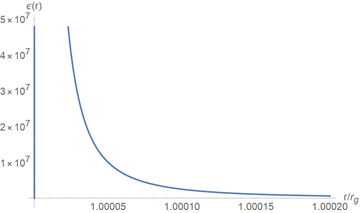
\includegraphics[width=0.45\textwidth]{scal-vec/scal-rg-ee-sec2-rg}}%
            \hspace{8pt}%
            %
            \subfloat[][]{%
                \label{fig:scal-rg-uu-sec2-rg}%
                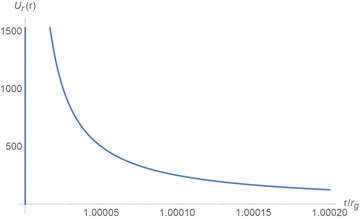
\includegraphics[width=0.45\textwidth]{scal-vec/scal-rg-uu-sec2-rg}}%
            \hspace{8pt}%
            %
            \subfloat[][]{%
                \label{fig:scal-rg-ee-sec2}%
                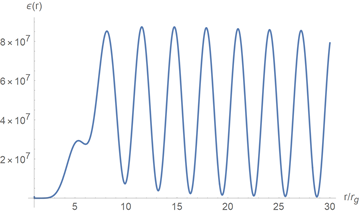
\includegraphics[width=0.45\textwidth]{scal-vec/scal-rg-ee-sec2}}%
            \hspace{8pt}%
            %
            \subfloat[][]{%
                \label{fig:scal-rg-uu-sec2}%
                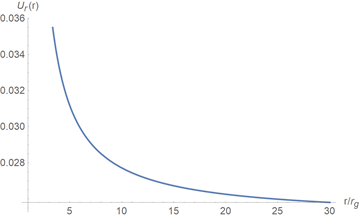
\includegraphics[width=0.45\textwidth]{scal-vec/scal-rg-uu-sec2}}%
            \hspace{8pt}%
            %
            \caption[]{Плотность (\subref{fig:scal-rg-ee-sec1}, \subref{fig:scal-rg-ee-sec2-rg}, \subref{fig:scal-rg-ee-sec2}) и поток энергии (радиальная компонента; \subref{fig:scal-rg-uu-sec1}, \subref{fig:scal-rg-uu-sec2-rg}, \subref{fig:scal-rg-uu-sec2}) $l=5$ моды первого бегущего решения в зависимости от радиуса в различных областях пространства при фиксированном угле $\theta = \pi/4$}%
            \label{fig:scal-ee-uu}%
        \end{figure}
        %
        \begin{figure}[h]
            \centering
            %
            \subfloat[][]{%
                \label{fig:scal-rg-ee-sec2-p2}%
                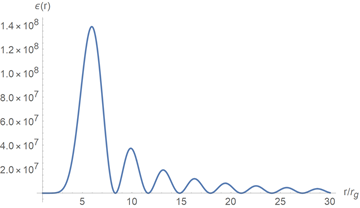
\includegraphics[width=0.45\textwidth]{scal-vec/scal-rg-ee-sec2-p2}}%
            \hspace{8pt}%
            %
            \subfloat[][]{%
                \label{fig:scal-rg-uu-sec2-p2}%
                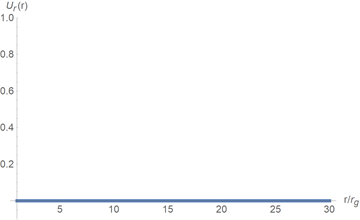
\includegraphics[width=0.45\textwidth]{scal-vec/scal-rg-uu-sec2-p2}}%
            \hspace{8pt}
            %
            \caption[]{Плотность \subref{fig:scal-rg-ee-sec2-p2} и поток энергии (радиальная компонента) \subref{fig:scal-rg-uu-sec2-p2} $l=5$ моды первого бегущего решения в зависимости от радиуса в области $r \gg r_g$ при фиксированном угле $\theta = \pi/2$. Поток энергии здесь полностью отсутствует~--- волны в данном направлении чисто стоячие}%
            \label{fig:scal-ee-uu-p2}%
        \end{figure}
        %
        Графики отражают тот факт, что в области $r < r_g$ волны бегущие, область $r = r_g + \varepsilon$ содержит в основном бегущие волны, область $r \gg r_g$ содержит практически только стоячие волны. В различных направлениях волны распространяются по-разному: при угле распространения $\theta = \pi/2$ волны чисто стоячие (при любом $r > 0$), по другим направлениям в них также присутствует и бегущая компонента. Более того, из-за сильной особенности в $r = r_g$, плотность энергии в данной точке стремится к бесконечности.

\subsection{Векторное поле}

    Наиболее важным векторным полем является электромагнитное поле. Лагранжиан электромагнитного поля имеет вид \cite{landau_v2}
    %
    \begin{equation*}
        \mathcal{L} = - \frac{1}{4} g^{ik} g^{jl} F_{ij} F_{kl} ,
    \end{equation*}
    %
    где
    %
    \begin{equation*}
        F_{ij} = A_{i;j} - A_{j;i} = A_{i,j} - A_{j,i} .
    \end{equation*}
    %
    Векторный 4-потенциал $A_i$ определяет скалярный потенциал $\varphi$, электрическое и магнитное поля $\vb{E}$ и $\vb{B}$:
    %
    \begin{equation*}
        A^i = \qty(\varphi, \vb{A}), \qquad
        \vb{E} = \dot{\vb{A}}, \qquad
        \vb{B} = \mathop{\mathbf{rot}}{\vb{E}} .
    \end{equation*}

    Калибровочное преобразование, не меняющее вариационных уравнений, допускает обращения скалярного потенциала в нуль \cite{landau_v2}. Здесь мы воспользуемся этим фактом для упрощения выкладок. Мы также рассматриваем исключительно свободное пространство, лишенное всякого вещества.

    Опять же, разделением переменных в вариационных уравнениях (см. напр. \cite{BurVas2019}) приходим к необходимому виду базовой, не зависящей от $\phi$ моды вектора $\vb{A}$ в любом сферически симметричном пространстве:
    %
    \begin{equation*}
        A_i(t,r,\theta) = \qty(Y_l(\theta) F_1(t,r),\ {Y'}_l(\theta) F_2(t,r),\ {Y'}_l(\theta) \sin(\theta) F_3(t,r))
    \end{equation*}
    %
    Здесь $Y_l(\theta) \equiv Y_l^0(\theta,\phi) = P_l(\cos\theta)$~--- те же, что и в случае скалярного поля. Моды с иным числом $-l \le m \le l$ могут быть сгенерированы из основного решения \enquote{механически} (см. напр. все тот же \cite{BurVas2019}) и здесь не рассматриваются.

    Прежде, чем приступать к анализу решений, необходимо сделать дополнительное упрощение. Оно связано с наличием двух независимых поляризаций векторного потенциала $\vb{A}$, которые, в свою очередь, определяются поведением компонент решений при отражении (замене $\phi \to -\phi$). Четная поляризация имеет вид $\vb{A} = (A^1, A^2, 0)$, нечетная~--- $\vb{A} = (0, 0, A^3)$. В вариационных уравнениях компонента $A^3$ определяется независимо от завязанных друг на друга компонент $A^1$ и $A^2$. Более того, нечетные гармоники формально переводятся в четные применением оператора $\Rot$ \cite{Vas2018a,BurVas2019}. Отсюда следует достаточность рассмотрения лишь только нечетных гармоник в силу их простоты и наглядности, а также \enquote{механического} пути получения из них четных, более сложно устроенных гармоник.

    Таким образом, с учетом всех сделанных упрощений исследуемая базовая гармоника приобретает вид:
    %
    \begin{equation*}
        A_i(t,r,\theta) = e^{-i t} w(r) \sin(\theta) P_l^1(\cos\theta) \qty(0,\,0,\,0,\,1).
    \end{equation*}

    Тензор энергии-импульса для векторного поля, полученный непосредственно из лагранжиана, оказывается несимметричным. Его можно привести к симметричному виду, пользуясь неоднозначностью его определения. Симметризованный тензор энергии-импульса выглядит следующим образом \cite{landau_v2}:
    %
    \begin{equation*}
        \mathcal{T}_{ik} = -g^{sk} g^{ij} g^{ml} F_{jm} F_{sl} + 1/4 g^{ik} g^{jl} g^{sm} F_{ml} F_{js} .
    \end{equation*}
    %
    Средние по периоду значения компонент вычисляются так же, как и в случае скалярного поля.

    \paragraph{Плоское пространство.}

        Вид функции $w(r)$ в плоском пространстве определяется из единственного нетривиального вариационного уравнения:
        %
        \begin{equation}\label{eq:vec-m-eq}
            2 r^2 w''(r) - 2 (l\,(l + 1) - r^2) w(r) = 0.
        \end{equation}
        %
        Решениями данного уравнения являются функции $w_{1,2}(r) = r\,h_{1,2}(r)$, где $h_{1,2}$~--- известные из скалярного случая функции Ганкеля первого и второго рода (\autoref{fig:vec-h12}). Данные бегущие волны также могут быть обращены в стоячие соответствующей комбинацией (сложением, вычитанием) функций $h_1(r)$ и $h_2(r)$.

        Поскольку функции Ганкеля убывают при $r \to \infty$ как первая степень $r$, компонента $A_3$ векторного потенциала не убывает на бесконечности. Это, однако, не мешает плотности энергии (бегущих волн) убывать на бесконечности (\autoref{fig:vec-ee}), причем, в отличие от скалярных волн, она монотонна по $r$ независимо от направления $\theta$. Направление определяет лишь предельное значение, к которому стремится плотность энергии. Поток энергии не зависит от $r$. Для стоячих волн картина почти аналогична скалярному случаю: плотность энергии исходит из нуля ($r = 0$), проходит свой первый максимум, а далее начинает осциллировать вокруг некоторого предельного уровня, определяемого направлением $\theta$. Здесь направление, опять же, определяет лишь уровень, к которому плотность энергии стремится, в отличие от скалярных волн, плотность энергии которых существенно видоизменяется от направления $\theta$ (осцилляции на бесконечности то увеличиваются по амплитуде, то уменьшаются; здесь амплитуда осцилляций почти неизменна, меняется лишь \enquote{базовый уровень} кривой плотности энергии). Поток энергии у стоячих волн, разумеется, отсутствует.
        %
        \begin{figure}[h]
            \centering
            %
            \subfloat[][]{%
                \label{fig:vec-h1}%
                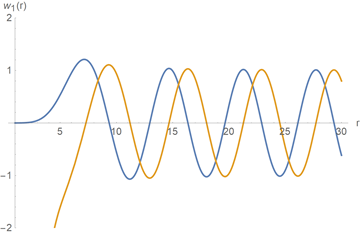
\includegraphics[width=0.45\textwidth]{scal-vec/vec-h1}}%
            \hspace{8pt}%
            %
            \subfloat[][]{%
                \label{fig:vec-h2}%
                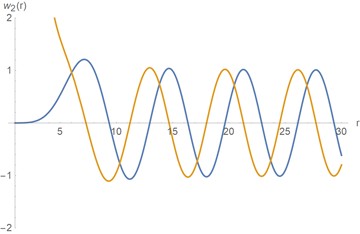
\includegraphics[width=0.45\textwidth]{scal-vec/vec-h2}}%
            \hspace{8pt}%
            %
            \caption[]{Два решения $w_{1,2}(r)$ в плоском пространстве при $l = 5$. Изображены действительная и мнимая части}%
            \label{fig:vec-h12}%
        \end{figure}
        %
        \begin{figure}[h]
            \centering
            %
            \subfloat[][]{%
                \label{fig:vec-h1-ee}%
                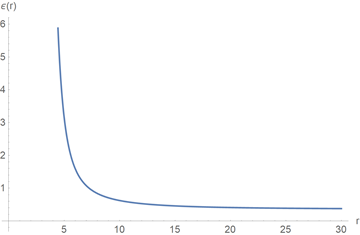
\includegraphics[width=0.45\textwidth]{scal-vec/vec-h1-ee}}%
            \hspace{8pt}%
            %
            \subfloat[][]{%
                \label{fig:vec-j1-ee}%
                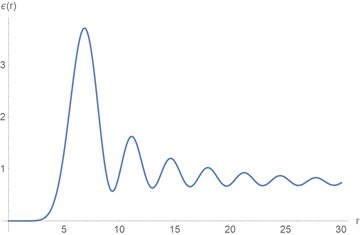
\includegraphics[width=0.45\textwidth]{scal-vec/vec-j1-ee}}%
            \hspace{8pt}%
            %
            \caption[]{Плотность энергии $l = 5$ моды \subref{fig:vec-h1-ee} бегущей, \subref{fig:vec-j1-ee} стоячей волны в направлении $\theta = -\pi/4$}%
            \label{fig:vec-ee}%
        \end{figure}

    \paragraph{Метрика Шварцшильда.}

        Радиальная компонента $w(r)$ в метрике Шварцшильда получается из вариационного уравнения:
        %
        \begin{gather}\label{eq:vec-sw-eq}
            w''(r) + \qty(-\frac{1}{r} + \frac{1}{r - r_g})\, w'(r) - \qty(\frac{l\,(l+1)}{r\, (r-r_g)} - \frac{r^2}{(r-r_g)^2})\, w(r) = 0.
        \end{gather}
        %
        Оно отличается от скалярного уравнения (\ref{eq:scal-sw-eq}) лишь знаком перед членом $1/r$, стоящим в скобках перед $w'(r)$. Этого, однако, достаточно, чтобы серьезно изменить характер решения. Стоит отметить, что, в отличие от скалярного случая, заменой $w(r) \to r v(r)$ в уравнении (\ref{eq:vec-sw-eq}) мы не приходим к уравнению (\ref{eq:vec-m-eq}), т.е. решение уравнения (\ref{eq:vec-sw-eq}) не есть произведение $r$ и решения уравнения (\ref{eq:vec-m-eq}). Хотя по внешнему виду решений может сложиться именно такое впечатление (\autoref{fig:vec-rg}, \autoref{fig:vec-rg2}).

        Очевидно, что регулярные особые точки, обнаруживаемые у данного уравнения, те же, что и в скалярном случае, т.е. $r = 0$ и $r = r_g$, однако показатели у особой точки $r = 0$ несколько отличаются: $\lambda_{1,2} = 0,2$ против $\lambda_{1,2} = 0$ в скалярном случае. Из \autoref{sec:deq_sing} известно, что если показатели особой точки отличаются на целое число, одно из решений может не существовать. Это и наблюдается в данном случае~--- решение с показателем $\lambda = 0$ является несостоятельным: невозможно определить значение всех коэффициентов ряда, которым решение должно выражаться.

        Опять же, решение в окрестности нуля не столь интересно, поскольку его область сходимости полностью перекрывается с областью сходимости решения в окрестности соседней особой точки. Относительно численной процедуры поиска решения замечания те же, поскольку тип уравнения остается таким же.

        Свойства решений здесь также в основном совпадают с таковыми в скалярном случае, за исключением того, что при $r \gg r_g$ волны не убывают пропорционально $r$, а имеют постоянную амплитуду. Также в области $r < r_g$ амплитуда волны уменьшается в направлении $r to 0$, однако, в точке $r = 0$ функция не обращается в нуль, как это может показаться на первый взгляд. Нарастание частоты волны при $r \to r_g$ (с обеих сторон) также имеет место. Преобладание действительной части над мнимой в зоне $r \gg r_g$ еще более выражено, чем в скалярном случае.
        %
        \begin{figure}[h]
            \centering
            %
            \subfloat[][]{%
                \label{fig:vec-rg-sec1}%
                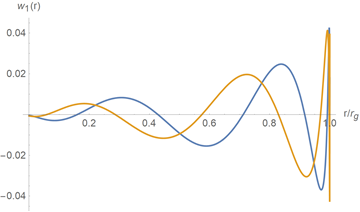
\includegraphics[width=0.45\textwidth]{scal-vec/vec-rg-sec1}}%
            \hspace{8pt}%
            %
            \subfloat[][]{%
                \label{fig:vec-rg-sec2}%
                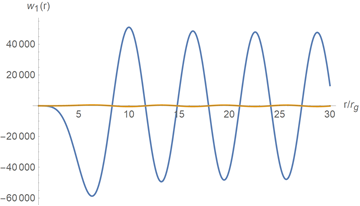
\includegraphics[width=0.45\textwidth]{scal-vec/vec-rg-sec2}}%
            \hspace{8pt}%
            %
            \subfloat[][]{%
                \label{fig:vec-rg-sec1-rg}%
                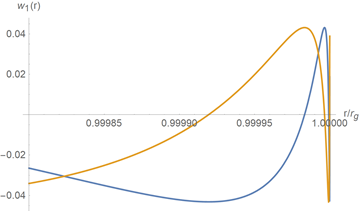
\includegraphics[width=0.45\textwidth]{scal-vec/vec-rg-sec1-rg}}%
            \hspace{8pt}%
            %
            \subfloat[][]{%
                \label{fig:vec-rg-sec2-rg}%
                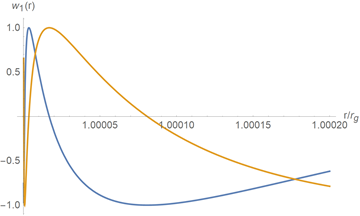
\includegraphics[width=0.45\textwidth]{scal-vec/vec-rg-sec2-rg}}%
            \hspace{8pt}%
            %
            \caption[]{Векторные решение $w_1(r)$ ($l = 5$, действительная и мнимая части) в различных областях:
                \subref{fig:vec-rg-sec1}~$r<r_g$,
                \subref{fig:vec-rg-sec2}~$r > r_g$,
                \subref{fig:vec-rg-sec1-rg}~$r = r_g - \varepsilon$,
                \subref{fig:vec-rg-sec2-rg}~$r = r_g + \varepsilon$}%
            \label{fig:vec-rg}%
        \end{figure}
        %
        \begin{figure}[h]
            \centering
            %
            \subfloat[][]{%
                \label{fig:vec-rg2-sec1}%
                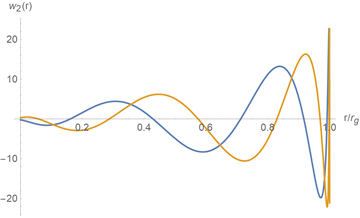
\includegraphics[width=0.45\textwidth]{scal-vec/vec-rg2-sec1}}%
            \hspace{8pt}%
            %
            \subfloat[][]{%
                \label{fig:vec-rg2-sec2}%
                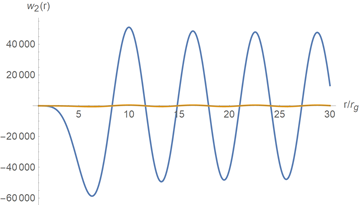
\includegraphics[width=0.45\textwidth]{scal-vec/vec-rg2-sec2}}%
            \hspace{8pt}%
            %
            \subfloat[][]{%
                \label{fig:vec-rg2-sec1-rg}%
                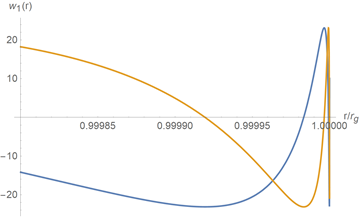
\includegraphics[width=0.45\textwidth]{scal-vec/vec-rg2-sec1-rg}}%
            \hspace{8pt}%
            %
            \subfloat[][]{%
                \label{fig:vec-rg2-sec2-rg}%
                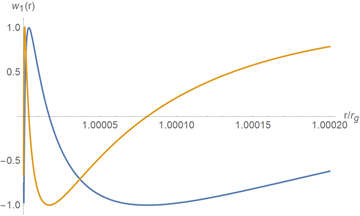
\includegraphics[width=0.45\textwidth]{scal-vec/vec-rg2-sec2-rg}}%
            \hspace{8pt}%
            %
            \caption[]{Векторные решение $w_2(r)$ ($l = 5$, действительная и мнимая части) в различных областях:
                \subref{fig:vec-rg2-sec1}~$r<r_g$,
                \subref{fig:vec-rg2-sec2}~$r > r_g$,
                \subref{fig:vec-rg2-sec1-rg}~$r = r_g - \varepsilon$,
                \subref{fig:vec-rg2-sec2-rg}~$r = r_g + \varepsilon$}%
            \label{fig:vec-rg2}%
        \end{figure}

        Энергетические характеристики волн (\autoref{fig:vec-ee-uu}) здесь довольно интересны. В области $r < r_g$ также, как и у скалярных волн в плоском пространстве, обнаруживается зависимость вида кривой плотности энергии от направления $\theta$. В частности, вблизи $r = r_g$ имеется энергетическая \enquote{яма}, отсутствующая лишь по некоторым выделенным направлениями $\theta$. Возле начала координат, в силу того, что решения там не обращаются в нуль, наблюдается сгибание кривой плотности энергии к вертикали $r = 0$. Поток энергии почти не меняется по форме относительно скалярных волн. Зависимость плотности энергии в остальных областях и потока энергии в большинстве областей от направления $\theta$ такая же, как у векторных волн в плоском пространстве.
        %
        \begin{figure}[h]
            \centering
            %
            \subfloat[][]{%
                \label{fig:vec-rg-ee-sec1}%
                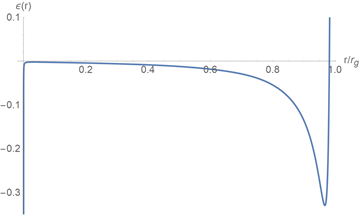
\includegraphics[width=0.45\textwidth]{scal-vec/vec-rg-ee-sec1}}%
            \hspace{8pt}%
            %
            \subfloat[][]{%
                \label{fig:vec-rg-uu-sec1}%
                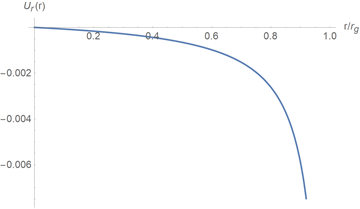
\includegraphics[width=0.45\textwidth]{scal-vec/vec-rg-uu-sec1}}%
            \hspace{8pt}%
            %
            \subfloat[][]{%
                \label{fig:vec-rg-ee-sec2-rg}%
                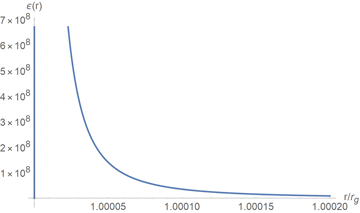
\includegraphics[width=0.45\textwidth]{scal-vec/vec-rg-ee-sec2-rg}}%
            \hspace{8pt}%
            %
            \subfloat[][]{%
                \label{fig:vec-rg-uu-sec2-rg}%
                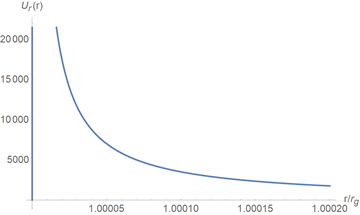
\includegraphics[width=0.45\textwidth]{scal-vec/vec-rg-uu-sec2-rg}}%
            \hspace{8pt}%
            %
            \subfloat[][]{%
                \label{fig:vec-rg-ee-sec2}%
                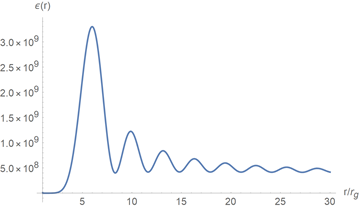
\includegraphics[width=0.45\textwidth]{scal-vec/vec-rg-ee-sec2}}%
            \hspace{8pt}%
            %
            \subfloat[][]{%
                \label{fig:vec-rg-uu-sec2}%
                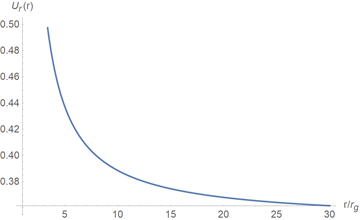
\includegraphics[width=0.45\textwidth]{scal-vec/vec-rg-uu-sec2}}%
            \hspace{8pt}%
            %
            \caption[]{Плотность (\subref{fig:vec-rg-ee-sec1}, \subref{fig:vec-rg-ee-sec2-rg}, \subref{fig:vec-rg-ee-sec2}) и поток энергии (радиальная компонента; \subref{fig:vec-rg-uu-sec1}, \subref{fig:vec-rg-uu-sec2-rg}, \subref{fig:vec-rg-uu-sec2}) $l=5$ моды первого векторного бегущего решения в зависимости от радиуса в различных областях пространства при фиксированном угле $\theta = -\pi/4$}%
            \label{fig:vec-ee-uu}%
        \end{figure}

\subsection{Анализ решений}

    В метрике Шварцшильда существенно меняется характер сферических гармоник тех или иных волн. Связано это, в первую очередь, с наличием особенности самой метрики~--- гравитационного радиуса~--- который делит пространство на две части: внутреннюю область (\enquote{под} гравитационным радиусом) и внешнюю область (\enquote{над} гравитационным радиусом). Волны должны видоизмениться таким образом, чтобы учитывать сложную структуру пространства.

    Второе, что бросается в глаза~--- смешанный характер самих волн: будучи бегущими в одной области пространства, они остаются стоячими в другой. Ни при каких условиях нельзя получить чисто бегущие волны над гравитационным радиусом. Также нельзя получить чисто стоячие решения во всем пространстве, поскольку под гравитационным радиусом в таком случае волны будут бегущими. Область под гравитационным радиусом в этом отношении является наиболее естественной, потому как там можно иметь оба типа волн, в то время как над гравитационным радиусом стоячая компонента неустранима.

    Третья интересная особенность волн~--- нарастание частоты при приближению к гравитационному радиусу. Иными словами, данной точке волны потребуется бесконечно большое время для пересечения горизонта событий. Под временем здесь понимается $t$~--- одна из четырех координат пространства-времени~--- время внешнего наблюдателя, а не собственное время данной точки волны. Исследование поведения волны в координатах, не содержащих особенности на гравитационном радиусе, представляет большой интерес, однако выходит за рамки данной работы.

    В остальном волны над гравитационным радиусом и стоячие волны в плоском пространстве обладают существенным сходством. Сходны и их энергетические характеристики.

\onlyinsubfile{
    \clearpage
    \phantomsection
    \addcontentsline{toc}{section}{Список литературы}
    \bibliographystyle{\docroot/../lib/doc/bib/utf8gosttu}
    \bibliography{\docroot/../lib/doc/bib/math,\docroot/../lib/doc/bib/physics}
}

\end{document}
